\chapter{Empirical Evaluation}

\section{Evaluation Over Synthetic Event Streams}

\section{Evaluation Over Real-word Event Streams}
\label{sec:results}
In this section, we evaluate our proposed system by analyzing the predictive performance and communication complexity  using real-world event streams provided by the datAcron project in the context of maritime monitoring. The used event streams describe critical points (i.e., synopses) of moving vessels trajectories, which are derived from raw AIS messages as described in \cite{synopses1}. In particular, for our evaluation experiments we used a data set of synopses that contains $4,684,444$ critical points of $5055$ vessels sailing in the Atlantic Ocean during the period from 1 October 2015 to 31 March 2016.

\par We used the synopses data set to generate a simulated stream of event tuples  i.e., \textit{(id, timestamp, longitude, latitude, annotation, speed, heading)}, which are processed by the system to attach an extra attribute \textit{type} that represents the event value,  where $type$ $\in \Sigma$,  and $ \Sigma= \Sigma_1=$$\{$\textit{VerySlow, Slow, Moving,  Sailing, Stopping}$\}$ , which is based on a discretization of the speed values. Or $\Sigma=\Sigma_2=$ $\{$\textit{stopStart, stopEnd, changeInSpeedStart, changeInSpeedEnd,  slowMotionStart, slowMotionEnd, gapStart, gapEnd, changeInHeading}$\}$, which is derived based on the values of the $annotation$ attribute that encodes the extracted trajectory movement events \cite{synopses1}. In our experiments, we monitor a pattern $\mathcal{P}_1=Sailing$ with $\Sigma_1$ that detects when the vessel is underway (sailing). Likewise, we test a second pattern  $\mathcal{P}_2=$\textit{changeInHeading; gapStart; gapEnd; changeInHeading} with $\Sigma_2$.


\subsection*{Experimental setup} We ran our experiments on single-node standalone Flink cluster deployed on an Ubuntu Server 17.04 with Intel(R) Core(TM) i7-7700 CPU @ 3.60GHz X 8 processors and 32GB RAM. We used Apache Flink v1.3.2 and Apache Kafka v0.10.2.1 for our tests.


\subsection*{Evaluation criteria} Our goal is to evaluate our distributed pattern prediction system, which enables the synchronization of prediction models (i.e., PMC models) on the distributed predictor nodes. Our proposed system can operate in three different modes of  protocols/schemes of models synchronization: \begin{enumerate}[]
	\item static scheme based on synchronizing the prediction models periodically every $b$ of input events in each stream, 
\item continuous, full synchronization for each incoming event (hypothetical), 
\item dynamic synchronization protocol based on making the predictors communicate their local prediction models periodically but only under condition that the divergence of the local models from a reference model exceeds a variance threshold $\Delta$ (recommended).  	   

\end{enumerate}
\par We compare our proposed system against the isolated prediction mode, in which models are computed on single streams only, and compare the predictive performance in terms of :
\begin{enumerate}[]
	
\item  $\mathit{precision} =$ $ \mathit{\frac{\#\ of\ correct\ predictions}{\#\ of\ total\ predictions}}$ is the fraction of the produced predictions that are correct (i.e., a full match occurred within the prediction interval).   

\item $\mathit{spread} =end(I) -start(I)$ is the width of the prediction interval $I$. 

\end{enumerate} 
\par Moreover, we study the communication cost by measuring the $\mathit{cumulative\ communication}$ that captures the number of messages, which are required to perform the distributed online learning modes to synchronize the prediction models. Next, we present the experimental results for the patterns  $\mathcal{P}_1=Sailing$ with an order of $m=2$, and   $\mathcal{P}_2=$\textit{changeInHeading; gapStart; gapEnd; changeInHeading} with first order $m=1$. All experiments are performed with setting the batch size to 100  ($b=100$), the variance threshold of 2 ($\Delta=2$), $80\%$ as PMC prediction threshold ($\theta_{fc}=80\%$), and 200 for the maximum spread.

\begin{figure}[h]
	
	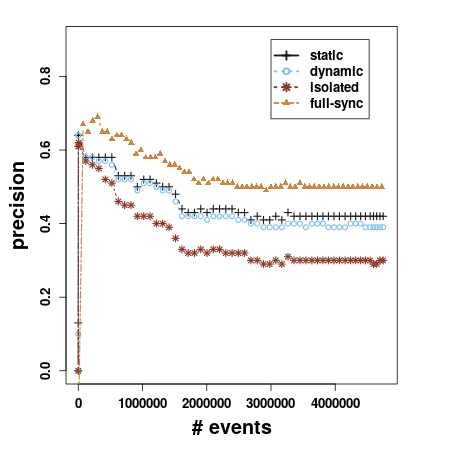
\includegraphics[width=\textwidth]{chapters/figures/precision_p1.png}
	
	\caption{Precision scores with respect to the number of input events over time for $\mathcal{P}_1$.}
	\label{fig:precsions}
\end{figure}

\subsection*{Experimental results} Figure ~\ref{fig:precsions} depicts the average precision scores of predictions models (one prediction model per vessel) of all synchronization modes for the first pattern $\mathcal{P}_1=Sailing$, namely, isolated without synchronization, continuous (full-sync), static, and our recommended approach based on the dynamic synchronization scheme. It can be clearly seen that all methods of distributed learning outperform the isolated prediction models. The hypothetical method of full continuous synchronization has the highest precision rates, while the static and dynamic synchronization schemes have close precision scores. Consequently, dynamic synchronization is not much weaker than the static synchronization, but requires much less communication, as explained below.
 

 
\par Figure ~\ref{fig:comm} provides the amount of the accumulated communication that is required by the three modes of the distributed online learning, while the isolated approach does not require any communication between the predictors. These results are shown  for $\mathcal{P}_1$.  As expected, a larger amount of communication is required for the continuous synchronization comparing to the static and dynamic approaches. Also, it can be seen that we can reduce the communication overhead by applying the dynamic synchronization protocol (a reduction by a factor of 100) comparing to the static synchronization scheme, even with a small variance threshold $\Delta=2$. Furthermore,  the dynamic  protocol is still preserving a close predictive performance to the static one (see Figure ~\ref{fig:precsions}).  Therefore, we will only consider the dynamic synchronization and the isolated approach in the  evaluation of the second pattern.

\begin{center}
	
	\begin{figure}[]
		
		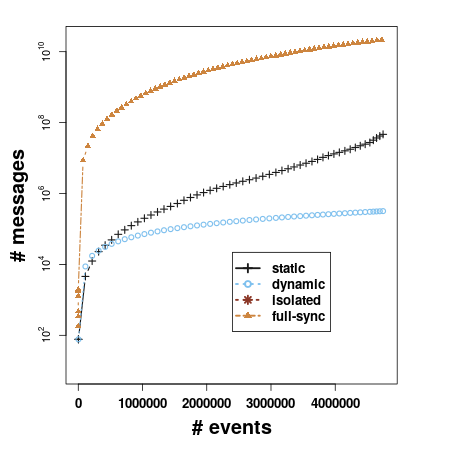
\includegraphics[width=\textwidth]{chapters/figures/messages_p1.png}
		
		\caption{Commutative communication with respect to the number of input events over time for $\mathcal{P}_1$.}
		\label{fig:comm}
	\end{figure}
\end{center}




\begin{center}
	
	\begin{figure}[]
		
		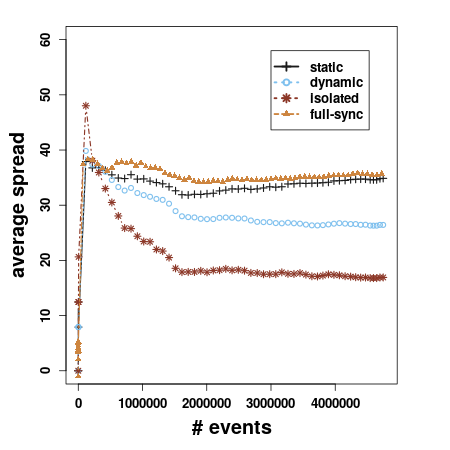
\includegraphics[width=\textwidth]{chapters/figures/spread_p1.png}
		
		\caption{Average spread value for $\mathcal{P}_1$.}
		\label{fig:spread}
	\end{figure}
\end{center}

 \begin{figure}[]
	
	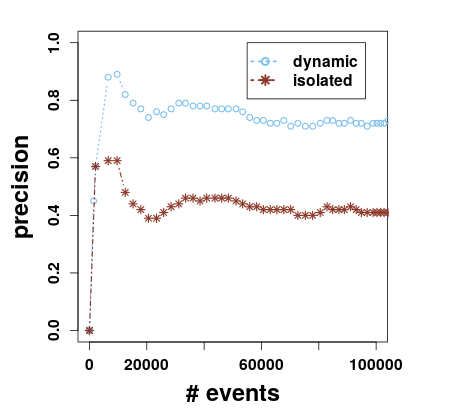
\includegraphics[width=\textwidth]{chapters/figures/precision_p2.png}
	
	\caption{Precision scores of $\mathcal{P}_2$  for \textit{PLEASURE CRAFT} vessels.}
	\label{fig:precsions_p2}
\end{figure}

\par In Figure ~\ref{fig:precsions}, we also noted that the precision is going down in a first phase and stabilizes then.  This seems to be counter-intuitive, as the models should improve when getting more data up to a certain point. For explanation, we have investigated the effect of the distributed synchronization of the prediction models on the average spread value, Figure  ~\ref{fig:spread}  shows the spread results for all approaches. It can be seen that the spread is higher for the distributed learning based methods comparing to the isolated approach. Furthermore, the average spread is decreasing over time until convergence, as result of confidence increase in the models. This may explain the drop in the precision scores from the beginning until reaching the convergence. We will investigate further in the interrelation between precision and spread in future work. 


\par For the second, more complex pattern ($\mathcal{P}_2$), we have found that the precision was worse for a distributed model generated over all vessels than in the model created for each vessel in isolation. This indicates that there is no  global model describing the behavior of all models consistently. However, when looking at specific groups of vessels, we achieved an improvement in terms of precision. As initial experiment, we only enable the synchronization of the prediction models associated with vessels that belong to the same vessel class. Currently, this change is technically performed by an extra filter step that passes only one type of vessels, while multiple runs of the system are required for all vessel types. For example, Figure ~\ref{fig:precsions_p2} shows the precision scores for vessels of class \textit{PLEASURE CRAFT}. An interesting observation is that the dynamic synchronization approach still has  a higher precision scores than the isolated approach. We will further investigate the effect of groupings and more patterns in future work.







%\par In Table ~\ref{tab:recall}, we present the mean of the recall scores for the both patterns in the all approaches It can be seen that the different approaches have a close recall scores, while the most frequent pattern ($\mathcal{P}_1$) has a lower recall than $\mathcal{P}_2$.
%
%\begin{table}[h]
%	\caption{Average recall for  $\mathcal{P}_1$ and $\mathcal{P}_2$.}
%	\label{tab:recall}
%	\begin{tabular}{lcc}
%		\toprule
%		Approach &Mean recall for $\mathcal{P}_1$ &Mean recall for $\mathcal{P}_2$\\
%		\midrule
%		isolated & 0.1707  &0.947 \\
%		static & 0.1754  &  0.960 \\
%		dynamic & 0.174  & 0.0.964 \\
%		full-sync & 0.1817  & 0.972 \\
%		\bottomrule
%	\end{tabular}
%\end{table}


 
